\documentclass[%
  aspectratio=169,
  9pt,
%   t,
%  USenglish,
ngerman,
%   dark,
  light,
  mathserif,
%   serif, 
  professionalfont,
%  handout,
%  affiliationinhead,
  affiliationintitlepagehead,
  titlegraphic,
  %% The following options would violate the CD rules!
   affiliation,
%   uselogos,
   navigationbar,
  progressbar,
%   seprules,
%   titleinhead,
]{beamer}




\usepackage{times}
\usepackage{epsfig}
\usepackage{graphicx}
\usepackage{amsmath}
\usepackage{amssymb}
\usepackage[utf8]{inputenc}
\usepackage{booktabs}
\setlength{\tabcolsep}{5pt}
\usepackage{subcaption}

\usepackage{appendix}
\usepackage{tummath}
\usepackage{tumtensors} % experimental
\usepackage{tumcolors}

\usepackage{pgfmath}
\newcommand\randmin{}
\newcommand\randmax{}
\newcommand\randmultof{}
\newcommand\setrand[4]%
{\def\randmin{#1}%
	\def\randmax{#2}%
	\def\randmultof{#3}%
	\pgfmathsetseed{#4}%
}
\newcommand\nextrand
{\pgfmathparse{int(int((rnd*(\randmax-\randmin+1)+\randmin)/\randmultof)*\randmultof)}%
	\xdef\thisrand{\pgfmathresult}%
}

% Include other packages here, before hyperref.

% If you comment hyperref and then uncomment it, you should delete
% egpaper.aux before re-running latex.  (Or just hit 'q' on the first latex
% run, let it finish, and you should be clear).
%\usepackage[breaklinks=true,bookmarks=false]{hyperref}


\usepackage[capitalize]{cleveref}
\usepackage[square,sort,comma,numbers]{natbib}

%% this hack seems to be nececessary due to incompatibilities of cvpr template and tikz... -> https://tex.stackexchange.com/questions/398223/tikz-gives-error-command-everyshipouthook-already-defined
\makeatletter
\@namedef{ver@everyshi.sty}{}
\makeatother
%% hackend

%{r\tikzsetnextfilenameawinput}

\newcommand{\rawtimeseries}[1]{

\begin{tikzpicture}[baseline=-2em, inner sep=0]

	\begin{axis}[
		thin,
		width=6cm,
		hide axis,
		height=3cm,
		ymin=0, ymax=1.4,
		no marks,  
		draw opacity=.8,
		smooth=0.01
	]
		 
	\addplot[b1color] table [x=t, y=B1, col sep=comma, forget plot] {images/example/#1};
	\addplot[b9color] table [x=t, y=B9, col sep=comma, forget plot] {images/example/#1};
	\addplot[b10color] table [x=t, y=B10, col sep=comma] {images/example/input.csv};
	
	\addplot[b11color] table [x=t, y=B11, col sep=comma, forget plot] {images/example/#1};
	\addplot[b12color] table [x=t, y=B12, col sep=comma] {images/example/#1};
	
	\addplot[b5color] table [x=t, y=B5, col sep=comma, forget plot] {images/example/#1};
	\addplot[b6color] table [x=t, y=B6, col sep=comma, forget plot] {images/example/#1};
	\addplot[b7color] table [x=t, y=B7, col sep=comma, forget plot] {images/example/#1};
	\addplot[b8color] table [x=t, y=B8, col sep=comma, forget plot] {images/example/#1};
	\addplot[b8Acolor] table [x=t, y=B8A, col sep=comma] {images/example/#1};
		
	\addplot[b2color] table [x=t, y=B2, col sep=comma, forget plot] {images/example/#1};
	\addplot[b3color] table [x=t, y=B3, col sep=comma, forget plot] {images/example/#1};
	\addplot[b4color] table [x=t, y=B4, col sep=comma] {images/example/#1};

	\end{axis}
	
\end{tikzpicture}
	
}

\usepackage{tikz}
\usepackage{pgfplots}
\usetikzlibrary{positioning, calc,arrows,arrows.meta, fit}
%\usetikzlibrary{arrows.meta,calc,decorations.markings,math,arrows.meta}
\usepgfplotslibrary{groupplots}
\usepgfplotslibrary{fillbetween}
\usepgfplotslibrary{statistics} % provides boxplots
\usepackage{xfrac}

\newcommand{\tp}{tp}
\newcommand{\tn}{tn}
\newcommand{\fp}{fp}
\newcommand{\fn}{fn}


\usepackage{tumcolors}
\usepackage{tummath}
\newcommand{\yhat}{\hat{\V{y}}}
\newcommand{\ycorrect}{\hat{y}^+}
\newcommand{\thetadelta}{\V{\Theta}_\delta}
\newcommand{\biasdelta}{b_\delta}
\newcommand{\biasclass}{\V{b}_\text{c}}
\newcommand{\thetaclass}{\V{\Theta}_\text{c}}
\newcommand{\thetafeat}{\V{\Theta}_\text{feat}}
\newcommand{\fclass}{f_\text{c}}
\newcommand{\fdelta}{f_\delta}
\newcommand{\ffeat}{f_\text{feat}}
\newcommand{\f}{f}

\newcommand{\rvtime}{T_c} 
\newcommand{\xuptot}{\M{X}_{\rightarrow t}} 
\newcommand{\deltauptot}{\delta_{\rightarrow t}} 
\newcommand{\tstop}{\ensuremath{t_\text{stop}}}
\newcommand{\meantstop}{\ensuremath{\bar{t}_\text{stop}}}
\usepackage[super]{nth}
\usepackage{mathtools}

\definecolor{evalcolor}{HTML}{3F3F3F}
\definecolor{traincolor}{HTML}{B98951}
\definecolor{validcolor}{HTML}{3F4BBE}

\colorlet{colortrain}{tumblue}
\colorlet{colorinfer}{tumblack}

\colorlet{earlinesscolor}{tumblue}
\colorlet{accuracycolor}{tumorange}

\colorlet{stdcolor}{tumbluelight}
\colorlet{mediancolor}{tumorange}
\colorlet{meancolor}{tumblue}

%\colorlet{b1color}{tumdiagramaubergine}
%\colorlet{b2color}{tumdiagramnavyblue}
%\colorlet{b3color}{tumdiagramturquoise}
%\colorlet{b4color}{tumdiagramgreen}
%\colorlet{b5color}{tumdiagramlimegreen}
%\colorlet{b6color}{tumdiagramyellow}
%\colorlet{b7color}{tumdiagramsand}
%\colorlet{b8color}{tumdiagramredorange}
%\colorlet{b8Acolor}{tumdiagramred}
%\colorlet{b9color}{tumblack}
%\colorlet{b10color}{tumblue}
%\colorlet{b11color}{tumdiagramdarkred}
%\colorlet{b12color}{tumorange}

% atmospheric bands
\colorlet{b1color}{tumblack}%tumdiagramaubergine
\colorlet{b9color}{tumblack}%tumblack
\colorlet{b10color}{tumblack}%tumblue

%visisble bands
\colorlet{b2color}{tumblue}%tumdiagramnavyblue
\colorlet{b3color}{tumblue}%tumdiagramturquoise
\colorlet{b4color}{tumblue}%tumdiagramgreen

% near infrared bands
\colorlet{b5color}{tumred}%tumdiagramlimegreen
\colorlet{b6color}{tumred}%tumdiagramyellow
\colorlet{b7color}{tumred}%tumdiagramsand
\colorlet{b8color}{tumred}%tumdiagramredorange
\colorlet{b8Acolor}{tumred}%tumdiagramred

% SWIR bands
\colorlet{b11color}{tumgreen}%tumdiagramdarkred
\colorlet{b12color}{tumgreen}%tumorange

\colorlet{epsilon0color}{tumorange}
\colorlet{epsilon1color}{tumblue}
\colorlet{epsilon10color}{tumblack}

\colorlet{meadowcolor}{tumbluemedium}
\colorlet{wbarleycolor}{tumbluedark}
\colorlet{corncolor}{tumorange}
\colorlet{wheatcolor}{tumgreen}
\colorlet{sbarleycolor}{tumred}
\colorlet{clovercolor}{tumturquoise}
\colorlet{triticalecolor}{tumsand}

\tikzstyle{rnn}=[draw,circle, inner sep=.1em]
\tikzstyle{norm}=[rounded corners,draw]
\tikzstyle{annot}=[rounded corners, fill=tumblue!20]
\tikzstyle{infer}=[-stealth, shorten >=.0em, shorten <=.0em, colorinfer]
\tikzstyle{loss}=[fill=tumblue!10, rounded corners, font=\small]
\tikzstyle{grad}=[colortrain]

\newcommand{\ptoffset}{\varepsilon}

\tikzstyle{test} = [thick]
\tikzstyle{train} = [thin, dotted]

\usepackage[inline]{enumitem}
\setenumerate{label=(\roman*),itemsep=3pt,topsep=3pt}

\setlength{\belowcaptionskip}{-10pt}
%\usepackage{titlesec}
%\titlespacing{\section}{0pt}{10pt}{3pt}

\usetikzlibrary{external}
\tikzexternalize[prefix=tikz/]
%\tikzexternalize
\tikzexternaldisable

\usepackage[eulergreek]{sansmath}
\pgfplotsset{
	y tick label style={/pgf/number format/.cd,%
		scaled y ticks = false,
		set thousands separator={},
		fixed},
	x tick label style={/pgf/number format/.cd,%
		scaled x ticks = false,
		set decimal separator={,},
		fixed},
	tick label style = {font=\sansmath\sffamily},
	every axis label = {
		font=\sansmath\sffamily},
	every axis/.append style={
		axis lines=left, 
		enlargelimits, 
		thick},
	legend style = {font=\sansmath\sffamily, draw=none, rounded corners, fill opacity=.5, text opacity=1},
	label style = {font=\sansmath\sffamily},
	grid style={line width=.1pt, draw=gray!10},
	major grid style={line width=.2pt,draw=tumgraylight},
}

%\let\tempone\itemize
%\let\temptwo\enditemize
%\renewenvironment{itemize}{\tempone\addtolength{\itemsep}{-.5\baselineskip}}{\temptwo}

\tikzstyle{circ} = [circle, draw=white, fill=tumblue, inner sep=1pt]
\newcommand{\fcn}{
	\begin{tikzpicture}[scale=0.2, rotate=0, baseline=-.25em, inner sep=1pt]
	\node[circ](a0) at (0,-1){};
	\node[circ](a1) at (0,0){};
	\node[circ](a2) at (0,1){};
	
	\node[circ](b0) at (1,-0.5){};
	\node[circ](b1) at (1,0.5){};
	
	\draw[-] (a0) -- (b0);
	\draw[-] (a1) -- (b0);
	\draw[-] (a2) -- (b0);
	
	\draw[-] (a0) -- (b1);
	\draw[-] (a1) -- (b1);
	\draw[-] (a2) -- (b1);
	
	\end{tikzpicture}
}


\newcommand{\earth}{
	\begin{tikzpicture}[baseline=-.25em, inner sep=0]
	\node{
\includegraphics[width=8mm]{images/icons/earth}};
	\end{tikzpicture}
}

\newcommand{\sat}{
	\begin{tikzpicture}[baseline=-.25em, inner sep=0]
	\node[rotate=270,anchor=center]{
\includegraphics[width=8mm]{images/icons/sat2}};
	\end{tikzpicture}
}

\newcommand{\hidden}[1]{
	\begin{tikzpicture}[scale=.1, baseline=-.25em]	
	%\draw[step=1.0,black,thin] (0,0) grid (#1,1);
	\foreach \i in {1,...,#1}{
		\node[circle, draw=white, fill=tumbluelight, inner sep=1pt] at (\i,0){};
	}
	\end{tikzpicture}
}

\newcommand{\drawvector}[1]{
	\begin{tikzpicture}[scale=.1, baseline=-.25em]	
	%\draw[step=1.0,black,thin] (0,0) grid (#1,1);
	\foreach \i in {1,...,#1}{
		\node[circ] at (\i,0){};
	}
	\end{tikzpicture}
}
\tikzstyle{proba} = [circle, draw=tumgray, inner sep=2.5pt, fill=tumorange]
\newcommand{\drawprobas}[5]{
	\begin{tikzpicture}[scale=.3, baseline=-.25em]	

	\node[proba, fill=tumblue!#1] at (0,-2){};
	\node[proba, fill=tumblue!#2] at (0,-1){};
	\node[proba, fill=tumblue!#3] at (0,-0){};
	\node[proba, fill=tumblue!#4] at (0,1){};
	\node[proba, fill=tumblue!#5] at (0,2){};
	\end{tikzpicture}
}

\newcommand{\vegetationsmodell}{
	\begin{tikzpicture}[scale=0.5, rotate=0, baseline=-.25em]
	\node[proba](a0) at (0,-1){};
	\node[proba](a1) at (0,0){};
	\node[proba](a2) at (0,1){};
	
	\node[proba](b0) at (1,-0.5){};
	\node[proba](b1) at (1,0.5){};
	
	\draw[-] (a0) -- (b0);
	\draw[-] (a1) -- (b0);
	\draw[-] (a2) -- (b0);
	
	\draw[-] (a0) -- (b1);
	\draw[-] (a1) -- (b1);
	\draw[-] (a2) -- (b1);
	
	\node[fit=(a0)(a2)(b1),draw,rounded corners](node name){};
	
	\end{tikzpicture}
}

\usepackage[utf8]{inputenc}
\usepackage[english, ngerman]{babel}
\usepackage[]{csquotes}

\usepackage{siunitx}

\sisetup{%
	mode = math,
	detect-family,
	detect-weight,  
	exponent-product = \cdot,
	number-unit-separator=\text{\,},
	output-decimal-marker={\text{,}},
	math-rm=\mathsf,
	text-rm=\sffamily,
}

\usepackage{animate}
%\usepackage{MnSymbol,wasysym}


%\newcommand{\org}{LMF}
% \newcommand{\org}{FPF}
%\newcommand{\coorg}{DLR}
\newcommand{\boldstruct}[1]{\textbf{\structure{#1}}}
\usetheme{TUM}
\usepackage{glossaries}
\usepackage{graphicx}
\usepackage{nth}
%\usepackage{natbib}
\usepackage[square,sort,comma,numbers]{natbib}
\bibliographystyle{abbrvnat}
%\setcitestyle{authoryear}%,open={((},close={))}

%\usepackage{tummath}
%\usepackage{tumtensors} % experimental
%\usepackage{tumcolors}
%%\usepackage{subfigure}
%%%\usepackage[noabbrev, capitalize]{cleveref}
%\usepackage{csvsimple}
%\usepackage{colortbl}
%%\usepackage{tabularx}
%\usepackage{multimedia}

\PassOptionsToPackage{cmyk}{xcolors}
	
\usepackage{booktabs}
\usepackage{contour}


%\usepackage{biblatex}
%\addbibresource{bib/ijgi}

\usepackage{pgfplots}
\usepgfplotslibrary{groupplots}
\usepackage{pgfplotstable}
\usepgfplotslibrary{dateplot}

%\usepgfplotslibrary{external}
%\tikzexternalize

\usepackage{booktabs}
\usepackage{array}
\newcolumntype{x}{l}
\newcolumntype{X}{>{}l}
\newcolumntype{v}[1]{>{\raggedright\hspace{0pt}}p{#1}}
\newcolumntype{V}[1]{>{\scriptsize\raggedright\hspace{0pt}}p{#1}}


\definecolor{fusionremovedcolor}{HTML}{00CA43}
\definecolor{fusionaddedcolor}{HTML}{FF00F7}
\definecolor{overlapcolor}{HTML}{FAC843}

\usepgfplotslibrary{external}
%\tikzexternalize
\tikzsetexternalprefix{tikz/}

\pgfdeclarelayer{background}
\pgfdeclarelayer{foreground}
\pgfsetlayers{background,main,foreground}

%\usetikzlibrary{mindmap}

%\usetikzlibrary{arrows} 
%\usetikzlibrary{backgrounds}
\usetikzlibrary{fit}
%\usetikzlibrary{shapes}
\usetikzlibrary{calc}
\usetikzlibrary{positioning}
\usetikzlibrary{matrix}
\usepackage[nodayofweek,level]{datetime}
%\usepackage{mwe}
%%
%
\usetikzlibrary{3d}
\tikzstyle{perspective3d}=[
x={(0.5cm,0.5cm)}, y={(1cm,0cm)}, z={(0cm,1cm)}]


\colorlet{traincolor}{tumbluelight}
\colorlet{validcolor}{tumbluedark}
\colorlet{evalcolor}{tumorange}

\colorlet{forwardcolor}{tumblue}
\colorlet{backwardcolor}{tumorange}

\colorlet{activationcolor}{tumblue}
\colorlet{gridcolor}{tumgraylight}
\colorlet{contextonecolor}{tumorange}
\colorlet{contexttwocolor}{tumorange!80}
\colorlet{contextthreecolor}{tumorange!60}
\colorlet{contextfourcolor}{tumorange!40}

% defaultvalue -> might be replaced later
\colorlet{tensorcolor}{forwardcolor}

\colorlet{classcolor}{tumivory}
\colorlet{encodercolor}{tumblue}
\colorlet{encodercolor}{tumred}

%\usepackage{media9}

% notation
\newcommand{\MWeight}{\ensuremath{\M{W}}}
\newcommand{\VBias}{\ensuremath{\V{b}}}
\newcommand{\VInput}{\DataVec}
\newcommand{\VHidden}{\ensuremath{\V{h}}}
\newcommand{\FActivation}{\ensuremath{\sigma}}
\newcommand{\VCellState}{\ensuremath{\V{c}}}
\newcommand{\VForgetGate}{\ensuremath{\V{f}}}
\newcommand{\VModulationGate}{\ensuremath{\V{j}}}
\newcommand{\VInputGate}{\ensuremath{\V{i}}}
\newcommand{\VOutputGate}{\ensuremath{\V{o}}}



\newcommand{\VResetGate}{\ensuremath{\V{r}}}
\newcommand{\VUpdateGate}{\ensuremath{\V{u}}}

%\newcommand{\concat}[2]{\VecDef{#1 \Vert #2}}
\newcommand{\concat}[2]{[#1\Vert#2]}

\newcommand{\Rin}[3]{\mathbb{R}^{[#1 \times #2 \times #3]}}
\newcommand{\Rinfloor}[3]{\mathbb{R}^{[#1]} \times \mathbb{R}^{[#2]} \times \mathbb{R}^{[#3]}}
\newcommand{\Rinfour}[4]{\mathbb{R}^{[#1 \times #2 \times #3 \times #4]}}

% kernel size of rnn convolution
\newcommand{\krnn}{k_{rnn}}
% kernel size of classification convolution
\newcommand{\kclass}{k_{class}}

\newcommand{\eg}{e.g., }
\newcommand{\ie}{i.e. }

%\newcommand{\classname}[1]{\texttt{#1}}
\newcommand{\classname}[1]{\textsl{#1}} % what about \textsl for classnames?
\newcommand{\cn}[1]{\classname{#1}} % short alias

\newcommand{\nutzungscn}[1]{\textsc{#1}} % stmelf Nutzungsklassen

\newcommand{\brand}[1]{\textsc{#1}}
\newcommand{\processing}[1]{\brand{#1}}
\newcommand{\satellite}[1]{\brand{#1}}
\newcommand{\band}[1]{\brand{#1}}

% https://tex.stackexchange.com/questions/167925/how-to-make-maths-equations-start-at-the-left
\newcommand{\mathleft}{\@fleqntrue\@mathmargin0pt}
\newcommand{\mathcenter}{\@fleqnfalse}

\usetikzlibrary{spy}

% \usepackage[ngerman]{babel} % if you get errors on compile: rm *aux *out *log *nav *snm *toc

\newcommand{\rastergrid}{
	\input{images/rastergrid.tikz}
}
\newcommand{\vectorgrid}{
	\input{images/vectorgrid.tikz}
}

%\setbeamersize{description width=0mm}

\mode<handout>{
  \usepackage{pgfpages}
% feel free to use one of these layouts
%   \pgfpagesuselayout{1 on 1}[a4paper,border shrink=5mm]
  \pgfpagesuselayout{2 on 1}[a4paper,border shrink=5mm]
%   \pgfpagesuselayout{3 on 1}[a4paper,border shrink=5mm]
%   \pgfpagesuselayout{4 on 1}[a4paper,border shrink=5mm]
%   \pgfpagesuselayout{2 on 1 landscape}[a4paper,border shrink=5mm]
%   
% you can also add room for notes, but then the widescreen aspect ratio messes up a little
%   \usepackage{handoutWithNotes}
%   \pgfpagesuselayout{1 on 1 with notes}[a4paper,border shrink=5mm]
%   \pgfpagesuselayout{2 on 1 with notes}[a4paper,border shrink=5mm]
%   \pgfpagesuselayout{3 on 1 with notes}[a4paper,border shrink=5mm]
%   \pgfpagesuselayout{4 on 1 with notes}[a4paper,border shrink=5mm]
%   \pgfpagesuselayout{1 on 1 with notes landscape}[a4paper,border shrink=5mm]
%   \pgfpagesuselayout{2 on 1 with notes landscape}[a4paper,border shrink=5mm]
}


\setbeamercovered{transparent}

%%%%%%%%%%%%%%%%%%%%%%%%%%%%%%%%%%%%%%%%%%%%%%%%%%%%%%%%%%%%%%%%%%%%%%%%%%%%%%%%%%%%%%%

%Convolutional-Recurrent Networks for Multi-temporal Classification
\title{Convolutional LSTMs for Cloud-Robust Classification \\ of Remote Sensing Imagery}
%\subtitle{NeurIPS 2018 Workshop on Spatiotemporal Modeling and Decision-making}
\subtitle{$\Phi$-week 2019}
\author[M. Rußwurm, M. Körner]{Marc Rußwurm, Marco Körner}
\institute[TUM]{Technical University of Munich\\Chair of Remote Sensing Technology\\Computer Vision Research Group\\\url{www.lmf.bgu.tum.de/vision}}

\date{13th September 2019, ESA ESRIN, Frascati, Italy}

\begin{document}

\begin{frame}[t]
  \titlepage
\end{frame}

{{\setbeamertemplate{background canvas}{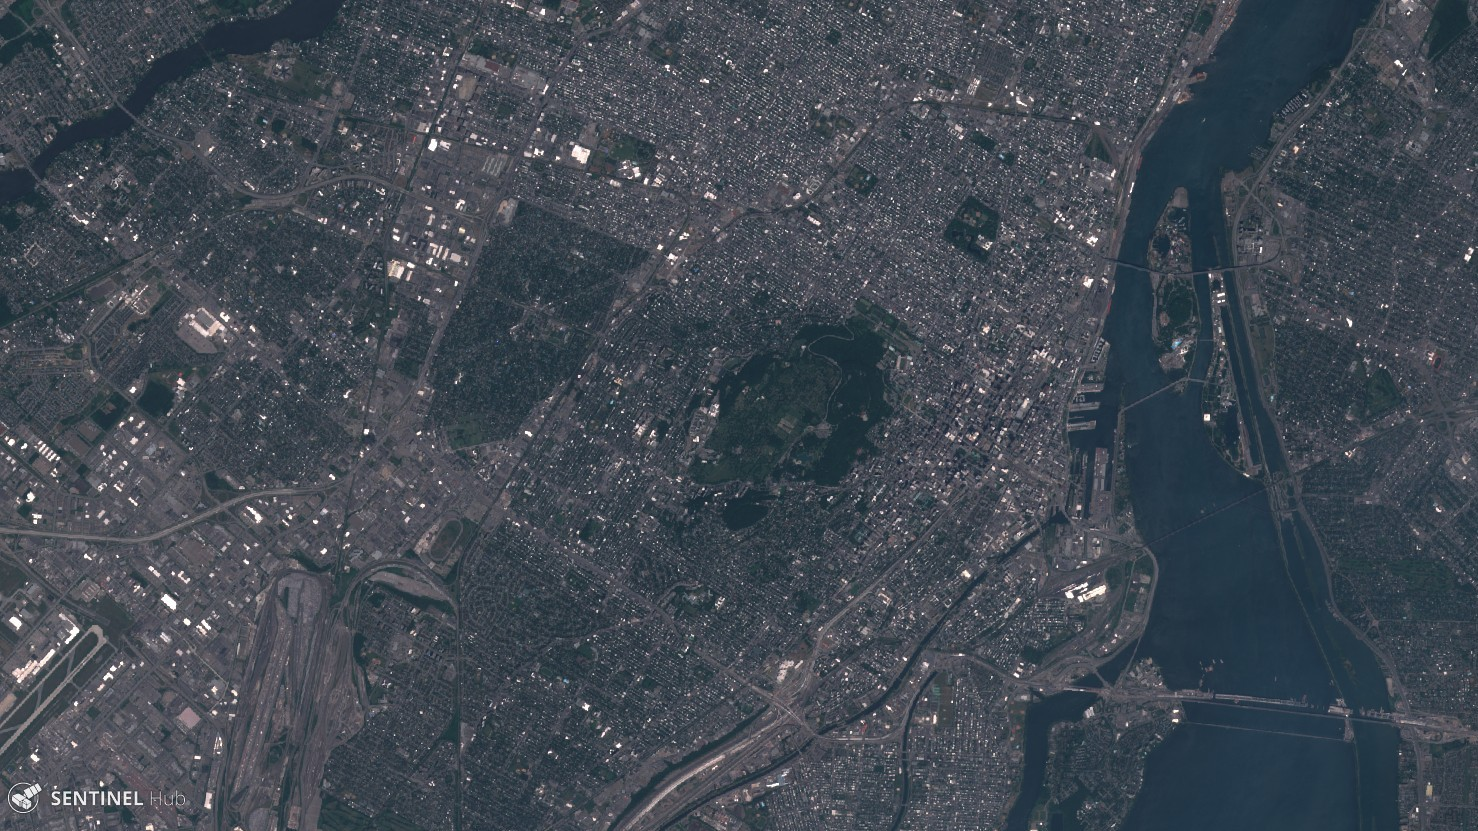
\includegraphics[width=\paperwidth]{images/cloudfree}}
\begin{frame}[plain]
%\frametitle{When we think of satellite images we picture this}
%%\centering\includegraphics[width=.75\textwidth]{images/montreal_satellite}
%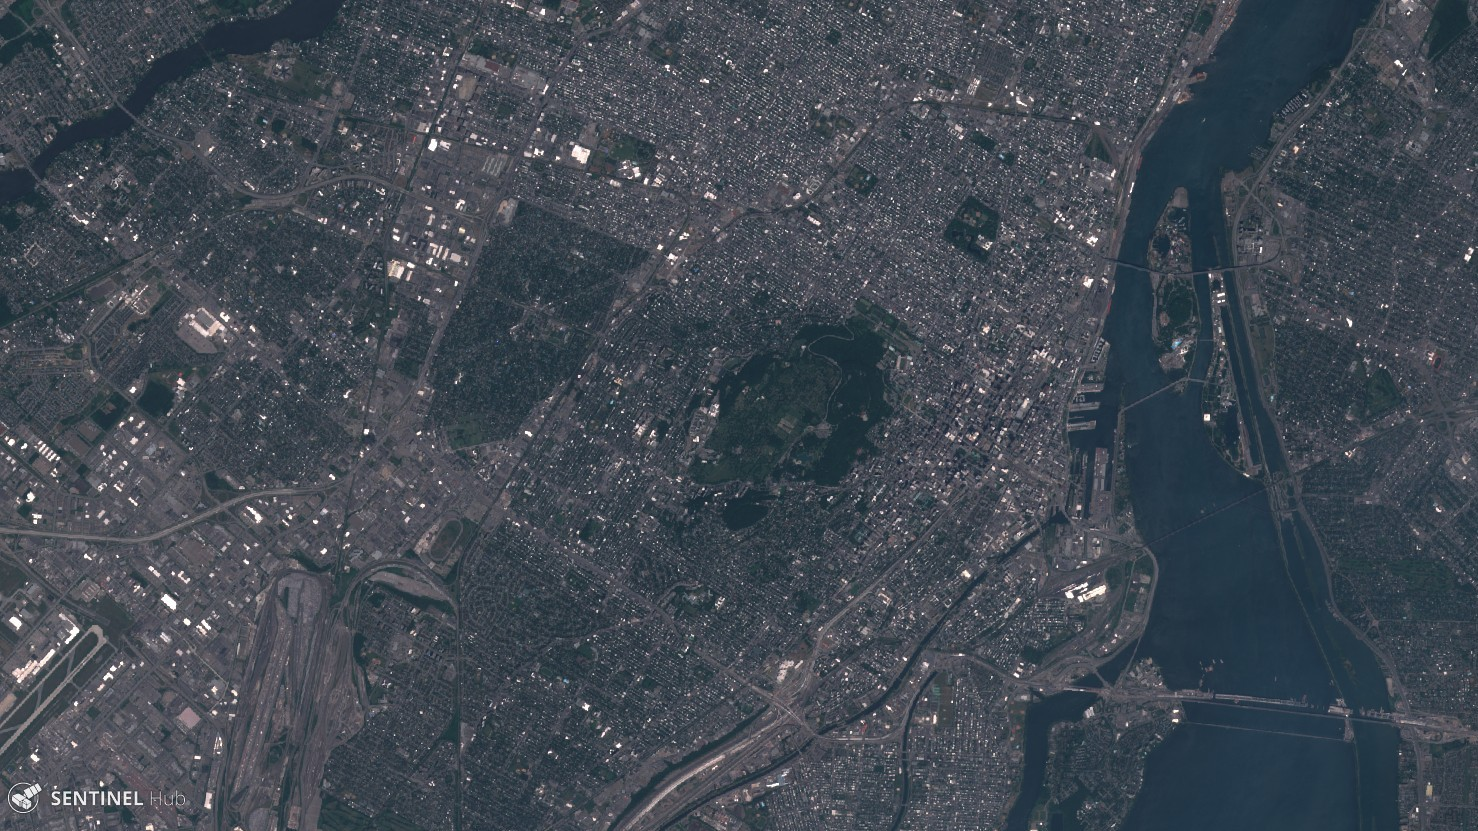
\includegraphics[width=\textwidth]{images/cloudfree}
\end{frame}
}

{\setbeamertemplate{background canvas}{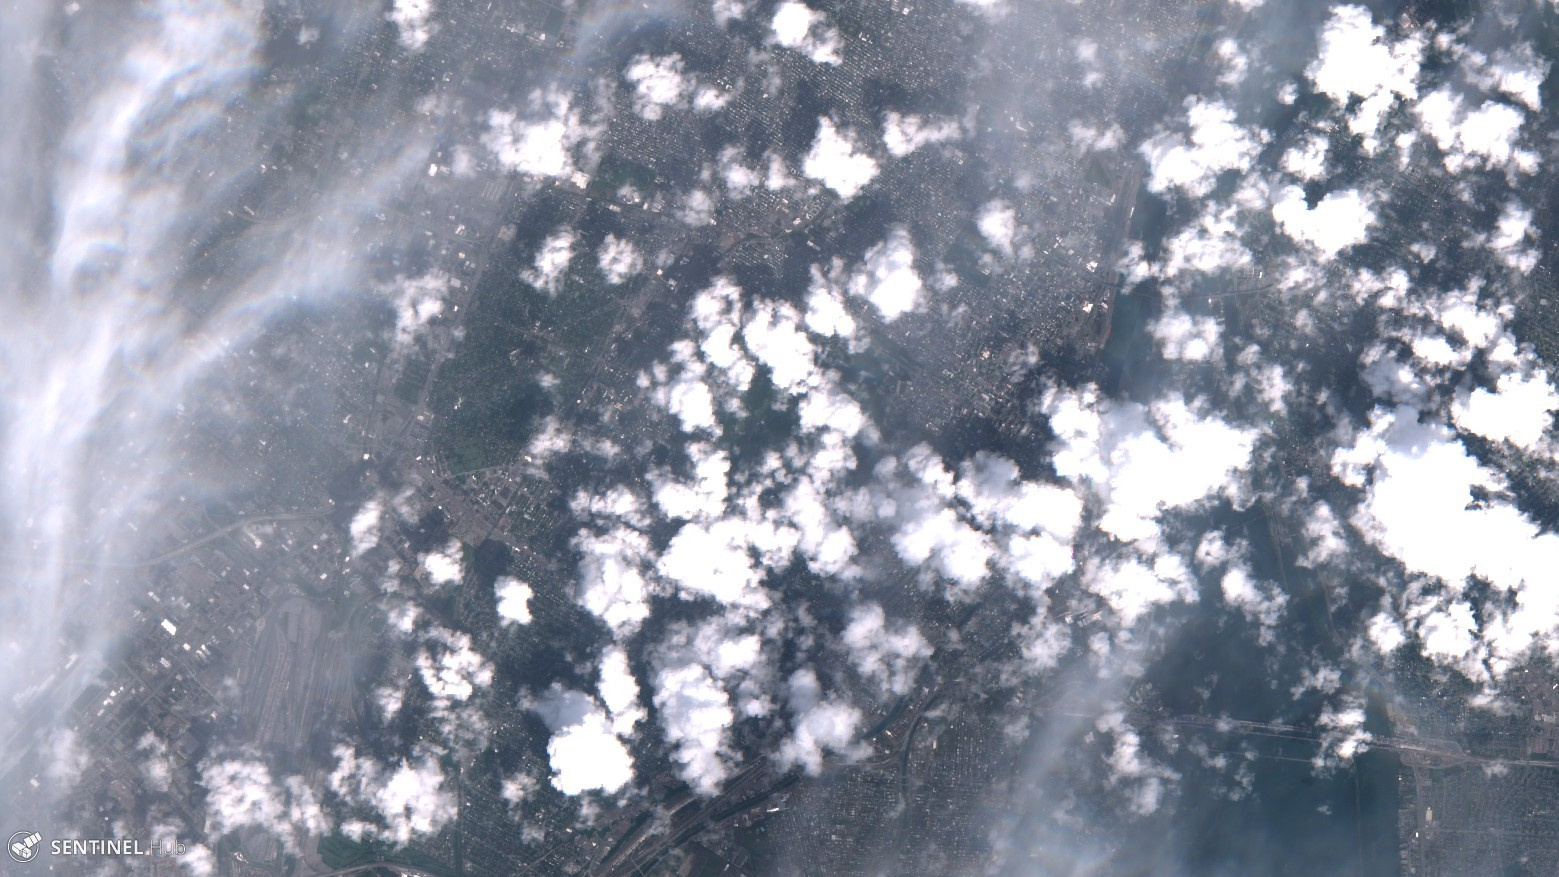
\includegraphics[width=\paperwidth]{images/clouds}}
	\begin{frame}[plain]
%		\frametitle{... however, ususally }
			
		
	%		\includegraphics[width=\textwidth]{images/cloud_airplane}
			
	\end{frame}
	
}

{\setbeamercolor{background canvas}{bg=tumbluedark}
	\begin{frame}[plain]
	
	\vspace{6em}
	\begin{center}
		\Huge\color{tumwhite}
		How should we deal with $
\includegraphics[width=2em]{images/icons/cloud2}^\ast$?
	\end{center}\color{white}
	\vspace{2em}
	\raggedleft \Large$^\ast$ ...and other noise in the data
	
	\vfill
%	\vspace{6em}
	\raggedleft{\small \color{tumgray}
	Icons made by Smashicons from www.flaticon.com
	}
\end{frame}
}

\begin{frame}
	\frametitle{Cloud coverage as spatiotemporal noise}
	\centering
	
	\def\imagewidth{1.5cm}
	
	
	\visible<1>{\includegraphics[width=\imagewidth]{images/activations/16494/x/x-0.png}}
	\visible<1>{\includegraphics[width=\imagewidth]{images/activations/16494/x/x-1.png}}
	\visible<1>{\includegraphics[width=\imagewidth]{images/activations/16494/x/x-2.png}}
	\visible<1>{\includegraphics[width=\imagewidth]{images/activations/16494/x/x-3.png}}
	\visible<1>{\includegraphics[width=\imagewidth]{images/activations/16494/x/x-4.png}}
	\visible<1,2>{\includegraphics[width=\imagewidth]{images/activations/16494/x/x-5.png}}
	\visible<1>{\includegraphics[width=\imagewidth]{images/activations/16494/x/x-6.png}}
	\visible<1>{\includegraphics[width=\imagewidth]{images/activations/16494/x/x-7.png}}
	\visible<1,2>{\includegraphics[width=\imagewidth]{images/activations/16494/x/x-8.png}}
	\visible<1>{\includegraphics[width=\imagewidth]{images/activations/16494/x/x-9.png}}
	\visible<1>{\includegraphics[width=\imagewidth]{images/activations/16494/x/x-10.png}}
	\visible<1>{\includegraphics[width=\imagewidth]{images/activations/16494/x/x-11.png}}
	\visible<1,2>{\includegraphics[width=\imagewidth]{images/activations/16494/x/x-12.png}}
	\visible<1,2>{\includegraphics[width=\imagewidth]{images/activations/16494/x/x-13.png}}
	\visible<1,2>{\includegraphics[width=\imagewidth]{images/activations/16494/x/x-14.png}}
	\visible<1,2>{\includegraphics[width=\imagewidth]{images/activations/16494/x/x-15.png}}
	\visible<1,2>{\includegraphics[width=\imagewidth]{images/activations/16494/x/x-16.png}}
	\visible<1>{\includegraphics[width=\imagewidth]{images/activations/16494/x/x-18.png}}
	\visible<1>{\includegraphics[width=\imagewidth]{images/activations/16494/x/x-19.png}}
	\visible<1,2>{\includegraphics[width=\imagewidth]{images/activations/16494/x/x-20.png}}
	\visible<1,2>{\includegraphics[width=\imagewidth]{images/activations/16494/x/x-21.png}}
	\visible<1>{\includegraphics[width=\imagewidth]{images/activations/16494/x/x-22.png}}
	\visible<1>{\includegraphics[width=\imagewidth]{images/activations/16494/x/x-23.png}}
	\visible<1>{\includegraphics[width=\imagewidth]{images/activations/16494/x/x-24.png}}
	\visible<1>{\includegraphics[width=\imagewidth]{images/activations/16494/x/x-25.png}}
	\visible<1>{\includegraphics[width=\imagewidth]{images/activations/16494/x/x-26.png}}
	\visible<1,2>{\includegraphics[width=\imagewidth]{images/activations/16494/x/x-27.png}}
	\visible<1>{\includegraphics[width=\imagewidth]{images/activations/16494/x/x-28.png}}
	\visible<1,2>{\includegraphics[width=\imagewidth]{images/activations/16494/x/x-29.png}}
	\visible<1>{\includegraphics[width=\imagewidth]{images/activations/16494/x/x-30.png}}
	\visible<1>{\includegraphics[width=\imagewidth]{images/activations/16494/x/x-31.png}}
	\visible<1,2>{\includegraphics[width=\imagewidth]{images/activations/16494/x/x-32.png}}
	\visible<1>{\includegraphics[width=\imagewidth]{images/activations/16494/x/x-33.png}}
%	
\end{frame}
%
%\begin{frame}
%\LARGE
%\centering
%\textbf{Filter this temporal noise by pre-classificaition?}
%\end{frame}

%\begin{frame}
%		
\usepgfplotslibrary{groupplots}

\tikzsetnextfilename{scl}
\begin{tikzpicture}

%\def\data{images/classhist/classHistograms.dat}
\def\data{images/clouds/scl2.csv}

\pgfplotsset{ every non boxed x axis/.append style={x axis line style=-},
	every non boxed y axis/.append style={y axis line style=-}}

\pgfplotsset{every axis/.append style={ybar=1pt, bar width=6pt, ymajorgrids}}
\pgfplotsset{every axis label/.append style={font=\footnotesize},tick pos=left,ylabel near ticks}
\pgfplotsset{every tick label/.append style={font=\scriptsize}}
%\pgfplotsset{every x tick label/.append style={rotate=90,anchor=east,font=\tiny}}
%   \pgfplotsset{every y tick label/.append style={/pgf/number format/.cd, fixed, precision=2, fixed zerofill,}}
%\tikzstyle{caption}=[font=\footnotesize, fill=tumwhite, fill opacity=.5, text opacity=1]


\begin{axis}[
%group style={
%	%       group size=1 by 4,
%	group size=1 by 1,
%	xlabels at=edge bottom,
%	xticklabels at=edge bottom,
%	ylabels at=edge left,
%	yticklabels at=edge left,
%	vertical sep=2pt,
%	horizontal sep=2pt
%},
width=\textwidth,
height=5cm,
%ymode=log,
%log origin=infty,
%     y dir=reverse,
%     scaled ticks=true,
%log ticks with fixed point,
%scaled x ticks=true,
axis lines=left,
xlabel={image acquisition dates},
ylabel={cloud coverage},
xlabel style={yshift=-2mm},
xmin=-.5,
xmax=46,
%xlabel=clouds,
ytick={1,10,25,50,100},
yticklabels={\SI{1}{\percent},\SI{10}{\percent},\SI{25}{\percent},\SI{50}{\percent},\SI{100}{\percent}},
xtick=data,
xticklabels={
	03. Jan,
	13. Jan,
	20. Jan,
	21. Jan,
	28. Jan,
	12. Feb,
	11. Mär,
	20. Mär,
	23. Mär,
	03. Apr,
	13 Apr.,
	19. Apr,
	22. Apr,
	29. Apr,
	02. Mai,
	10. Mai,
	22. Mai,
	29. Mai,
	08. Jun,
	18. Jun,
	28. Jan,
	02. Jul,
	14. Jul,
	18. Jul,
	21. Jul,
	28. Jul,
	30. Jul,
	07. Aug,
	17. Aug,
	20. Aug,
	28. Aug,
	21. Aug,
	09. Sep.,
	12. Sep..,
	18. Sep.,
	26. Sep.,
	29. Sep.,
	09. Okt.,
	18. Okt.,
	28. Okt.,
	09. Nov.,
	15. Nov.,
	18. Nov.,
	28. Nov.,
	06. Dez.,
	08. Dez.
},
axis on top
];

\addplot[
%       draw=tumblue,
draw=none,
fill=tumblue,rounded corners=.5pt
] table [col sep=comma, x=id, y=cloudpercent] {\data};


\end{axis}
\end{tikzpicture}
%\end{frame}


\input{images/overviewgraphs.tikz}

\begin{frame}<presentation:0>

\frametitle{Detecting Clouds is rarely the main objective}
\LARGE
\centering\figcloudfilteringpipeline

\end{frame}

%


%\begin{frame}<presentation:1>
%
%\frametitle{Introducing a model to pre-classify clouds?}
%\LARGE
%\centering\figcloudfilteringpipeline
%
%\end{frame}

%\begin{frame}
%\frametitle{Clouds classification works very well...}
%
%\includegraphics[width=\textwidth]{images/Li18_clouds}
%
%\texttt{\small Li, Z., Shen, H., Cheng, Q., Liu, Y., You, S., \& He, Z. (2018). Deep learning based cloud detection for remote sensing images by the fusion of multi-scale convolutional features. arXiv preprint arXiv:1810.05801.}
%\end{frame}
%
%\begin{frame}<presentation:2>
%
%\frametitle{Identifying clouds is rarely the main objective!}
%\LARGE
%\centering\figcloudfilteringpipeline
%
%\end{frame}

\begin{frame}
	\frametitle{Common Filtering/Preprocessing Algorithms work quite well}
	
	\begin{columns}
		\column{.5\textwidth}
		\begin{itemize}
			\item FMask
			\item MAJA
			\item Sen2Cor (F-Mask)
			\item supervised cloud classification e.g., CNNs
			\item unsupervised cloud clustering? {\small Go FDL!}
		\end{itemize}
		\column{.5\textwidth}
	
	\end{columns}
\end{frame}

\begin{frame}
\frametitle{End-to-End Learning of Deep Neural Networks}
\centering

\begin{tikzpicture}[node distance=.1em]
\node[font=\huge, label=above:\small $f_{\theta}$](veg) at (0,0){\vegetationsmodell};

\node[font=\huge,right=0em of veg, inner sep=0](bopen){$\Bigg($};
\node[right=.1em of veg, inner sep=0,label=below:Satellitendaten](input){\rawtimeseries{prep77770412.csv}};
\node[font=\huge, right=-.5em of input, inner sep=0](bopen){$\Bigg)$};

\node[left= of veg, font=\huge](equals){$=$};

\visible<1-5>{
	
	\node[left= of equals, label=below:$\yhat$](probas){\drawprobas{10}{30}{10}{20}{10}};
	%\node[left= of probas, font=\huge](arrow){$\leftarrow$};
	%\node[left= of arrow, font=\huge](probas){Mais};
}

\visible<5>{\node[left= of equals, label=below:$\yhat$](probas){\drawprobas{20}{30}{50}{20}{30}};}
\visible<6>{\node[left= of equals, label=below:$\yhat$](probas){\drawprobas{30}{40}{30}{50}{20}};}
\visible<7>{\node[left= of equals, label=below:$\yhat$](probas){\drawprobas{20}{20}{20}{80}{10}};}
\visible<8>{\node[left= of equals, label=below:$\yhat$](probas){\drawprobas{10}{30}{10}{100}{10}};}

\visible<2-8>{\node[left= 5em of probas, label=below:$\V{y}$](gt){\drawprobas{0}{0}{0}{100}{0}};}

\visible<3-8>{\draw[stealth-stealth] (gt) -- node[midway,above](loss){$\mathcal{L}(\V{y},\yhat)$} (probas);}

\visible<4-8>{\draw[-stealth] (loss)  to [out=60,in=135,looseness=1] node[midway,above]{$\theta \leftarrow \theta - \frac{\partial \mathcal{L}}{\partial \theta}$} (veg);}

\visible<9>{
	\node[left= of equals, label=below:scores](probas){\drawprobas{10}{30}{10}{100}{10}};
	\node[left= of probas, font=\huge](arrow){$\leftarrow$};
	\node[left= of arrow, font=\huge](probas){Mais};
}

%\visible<6>{
%\node[font=\bfseries\huge](e1) at (-3.4,-2.5){End};
%\node[font=\bfseries\huge](to) at (0,-2.5){to};
%\node[font=\bfseries\huge](e2) at (3.4,-2.5){End};
%\draw (e1) -- (to) -- (e2);
%}


\end{tikzpicture}

%	\begin{equation*}
%	\drawprobas = \drawprobas = \vegetationsmodell(\V{X}_t,\V{X}_{t+1},\V{X}_{t+2})
%	\end{equation*}


\end{frame}

\colorlet{attentioncolor}{tumred}
\newcommand{\attention}{%
	\only<1,2>{%
		\begin{tikzpicture}[scale=0.6]
		\node[draw=attentioncolor, circle, fill=attentioncolor, fill opacity=.4, text opacity=1, font=\small, inner sep=.2em](a) at (1,0){.2};
		\node[draw=attentioncolor, circle, fill=attentioncolor, fill opacity=.8, text opacity=1, font=\small, inner sep=.2em](b) at (2,0){.4};
		\node[draw=attentioncolor, circle, fill=attentioncolor, fill opacity=.2, text opacity=1, font=\small, inner sep=.2em](c) at (3,0){.1};
		\node[draw=attentioncolor, circle, fill=attentioncolor, fill opacity=.6, text opacity=1, font=\small, inner sep=.2em](d) at (4,0){.3};
		\end{tikzpicture}
	}%
	\only<3>{%
		\begin{tikzpicture}[scale=0.4]
		\node[draw=attentioncolor, circle, fill=attentioncolor, fill opacity=.4, text opacity=1, font=\small, inner sep=.2em](a) at (1,0){};
		\node[draw=attentioncolor, circle, fill=attentioncolor, fill opacity=.8, text opacity=1, font=\small, inner sep=.2em](b) at (2,0){};
		\node[draw=attentioncolor, circle, fill=attentioncolor, fill opacity=.2, text opacity=1, font=\small, inner sep=.2em](c) at (3,0){};
		\node[draw=attentioncolor, circle, fill=attentioncolor, fill opacity=.6, text opacity=1, font=\small, inner sep=.2em](d) at (4,0){};
		
		\node[draw=attentioncolor, circle, fill=attentioncolor, fill opacity=.4, text opacity=1, font=\small, inner sep=.2em](a) at (1,1){};
		\node[draw=attentioncolor, circle, fill=attentioncolor, fill opacity=.8, text opacity=1, font=\small, inner sep=.2em](b) at (2,1){};
		\node[draw=attentioncolor, circle, fill=attentioncolor, fill opacity=.2, text opacity=1, font=\small, inner sep=.2em](c) at (3,1){};
		\node[draw=attentioncolor, circle, fill=attentioncolor, fill opacity=.6, text opacity=1, font=\small, inner sep=.2em](d) at (4,1){};
		
		\node[draw=attentioncolor, circle, fill=attentioncolor, fill opacity=.4, text opacity=1, font=\small, inner sep=.2em](a) at (1,2){};
		\node[draw=attentioncolor, circle, fill=attentioncolor, fill opacity=.8, text opacity=1, font=\small, inner sep=.2em](b) at (2,2){};
		\node[draw=attentioncolor, circle, fill=attentioncolor, fill opacity=.2, text opacity=1, font=\small, inner sep=.2em](c) at (3,2){};
		\node[draw=attentioncolor, circle, fill=attentioncolor, fill opacity=.6, text opacity=1, font=\small, inner sep=.2em](d) at (4,2){};
		
		\node[draw=attentioncolor, circle, fill=attentioncolor, fill opacity=.4, text opacity=1, font=\small, inner sep=.2em](a) at (1,3){};
		\node[draw=attentioncolor, circle, fill=attentioncolor, fill opacity=.8, text opacity=1, font=\small, inner sep=.2em](b) at (2,3){};
		\node[draw=attentioncolor, circle, fill=attentioncolor, fill opacity=.2, text opacity=1, font=\small, inner sep=.2em](c) at (3,3){};
		\node[draw=attentioncolor, circle, fill=attentioncolor, fill opacity=.6, text opacity=1, font=\small, inner sep=.2em](d) at (4,3){};
		\end{tikzpicture}
	}%
}

\colorlet{valuecolor}{tumblue}
\newcommand{\attnv}{%
	\only<1,2>{%
		\begin{tikzpicture}[scale=0.6]
		\node[draw=valuecolor, circle, fill=valuecolor, fill opacity=.2, text opacity=1, font=\small, inner sep=.2em](a) at (0, 1){.2};
		\node[draw=valuecolor, circle, fill=valuecolor, fill opacity=.1, text opacity=1, font=\small, inner sep=.2em](b) at (0, 2){.1};
		\node[draw=valuecolor, circle, fill=valuecolor, fill opacity=.3, text opacity=1, font=\small, inner sep=.2em](c) at (0, 3){.3};
		\node[draw=valuecolor, circle, fill=valuecolor, fill opacity=.4, text opacity=1, font=\small, inner sep=.2em](d) at (0, 4){.4};
		\end{tikzpicture}
	}%
	\only<3>{%
		\begin{tikzpicture}[scale=0.4]
		\node[draw=valuecolor, circle, fill=valuecolor, fill opacity=.2, text opacity=1, font=\small, inner sep=.2em](a) at (0, 1){};
		\node[draw=valuecolor, circle, fill=valuecolor, fill opacity=.1, text opacity=1, font=\small, inner sep=.2em](b) at (0, 2){};
		\node[draw=valuecolor, circle, fill=valuecolor, fill opacity=.3, text opacity=1, font=\small, inner sep=.2em](c) at (0, 3){};
		\node[draw=valuecolor, circle, fill=valuecolor, fill opacity=.4, text opacity=1, font=\small, inner sep=.2em](d) at (0, 4){};
		
		\node[draw=valuecolor, circle, fill=valuecolor, fill opacity=.2, text opacity=1, font=\small, inner sep=.2em](a) at (1, 1){};
		\node[draw=valuecolor, circle, fill=valuecolor, fill opacity=.1, text opacity=1, font=\small, inner sep=.2em](b) at (1, 2){};
		\node[draw=valuecolor, circle, fill=valuecolor, fill opacity=.3, text opacity=1, font=\small, inner sep=.2em](c) at (1, 3){};
		\node[draw=valuecolor, circle, fill=valuecolor, fill opacity=.4, text opacity=1, font=\small, inner sep=.2em](d) at (1, 4){};
		\end{tikzpicture}
	}%
}

\colorlet{attentionoutcolor}{tumbluedark}
\newcommand{\attnout}{%
	\only<1,2>{%
		\begin{tikzpicture}[scale=0.6]
		\node[draw=tumblack, circle, fill=attentionoutcolor, text=white, text opacity=1, font=\small, inner sep=.2em](d) at (0,0){.27};
		\end{tikzpicture}
	}	
	\only<3>{%
		\begin{tikzpicture}[scale=0.4]
			\node[draw=tumblack, circle, fill=attentionoutcolor, text=white, text opacity=1, font=\small, inner sep=.2em](d) at (0,0){};
			\node[draw=tumblack, circle, fill=attentionoutcolor, text=white, text opacity=1, font=\small, inner sep=.2em](d) at (0,1){};
			\node[draw=tumblack, circle, fill=attentionoutcolor, text=white, text opacity=1, font=\small, inner sep=.2em](d) at (0,2){};
			\node[draw=tumblack, circle, fill=attentionoutcolor, text=white, text opacity=1, font=\small, inner sep=.2em](d) at (0,3){};
			
			\node[draw=tumblack, circle, fill=attentionoutcolor, text=white, text opacity=1, font=\small, inner sep=.2em](d) at (1,0){};
			\node[draw=tumblack, circle, fill=attentionoutcolor, text=white, text opacity=1, font=\small, inner sep=.2em](d) at (1,1){};
			\node[draw=tumblack, circle, fill=attentionoutcolor, text=white, text opacity=1, font=\small, inner sep=.2em](d) at (1,2){};
			\node[draw=tumblack, circle, fill=attentionoutcolor, text=white, text opacity=1, font=\small, inner sep=.2em](d) at (1,3){};
		\end{tikzpicture}
	}%
}

\colorlet{keycolor}{tumgreen}
\newcommand{\attnkey}{
	\only<1,2>{%
		\begin{tikzpicture}[scale=0.6]
			\node[draw=keycolor, circle, fill=keycolor, fill opacity=.2, text opacity=1, font=\small, inner sep=.2em](a) at (0, 0){.2};
			\node[draw=keycolor, circle, fill=keycolor, fill opacity=.1, text opacity=1, font=\small, inner sep=.2em](b) at (1, 0){.1};
			\node[draw=keycolor, circle, fill=keycolor, fill opacity=.3, text opacity=1, font=\small, inner sep=.2em](c) at (2, 0){.3};
			\node[draw=keycolor, circle, fill=keycolor, fill opacity=.4, text opacity=1, font=\small, inner sep=.2em](d) at (3, 0){.4};
			
			\node[draw=keycolor, circle, fill=keycolor, fill opacity=.2, text opacity=1, font=\small, inner sep=.2em](a) at (0, 1){.2};
			\node[draw=keycolor, circle, fill=keycolor, fill opacity=.1, text opacity=1, font=\small, inner sep=.2em](b) at (1, 1){.1};
			\node[draw=keycolor, circle, fill=keycolor, fill opacity=.3, text opacity=1, font=\small, inner sep=.2em](c) at (2, 1){.3};
			\node[draw=keycolor, circle, fill=keycolor, fill opacity=.4, text opacity=1, font=\small, inner sep=.2em](d) at (3, 1){.4};
		\end{tikzpicture}
	}
	\only<3>{%
		\begin{tikzpicture}[scale=0.4]
		\node[draw=keycolor, circle, fill=keycolor, fill opacity=.2, text opacity=1, font=\small, inner sep=.2em](a) at (0, 0){};
		\node[draw=keycolor, circle, fill=keycolor, fill opacity=.1, text opacity=1, font=\small, inner sep=.2em](b) at (1, 0){};
		\node[draw=keycolor, circle, fill=keycolor, fill opacity=.3, text opacity=1, font=\small, inner sep=.2em](c) at (2, 0){};
		\node[draw=keycolor, circle, fill=keycolor, fill opacity=.4, text opacity=1, font=\small, inner sep=.2em](d) at (3, 0){};
		
		\node[draw=keycolor, circle, fill=keycolor, fill opacity=.2, text opacity=1, font=\small, inner sep=.2em](a) at (0, 1){};
		\node[draw=keycolor, circle, fill=keycolor, fill opacity=.1, text opacity=1, font=\small, inner sep=.2em](b) at (1, 1){};
		\node[draw=keycolor, circle, fill=keycolor, fill opacity=.3, text opacity=1, font=\small, inner sep=.2em](c) at (2, 1){};
		\node[draw=keycolor, circle, fill=keycolor, fill opacity=.4, text opacity=1, font=\small, inner sep=.2em](d) at (3, 1){};
		
		\node[draw=keycolor, circle, fill=keycolor, fill opacity=.2, text opacity=1, font=\small, inner sep=.2em](a) at (0, 2){};
		\node[draw=keycolor, circle, fill=keycolor, fill opacity=.1, text opacity=1, font=\small, inner sep=.2em](b) at (1, 2){};
		\node[draw=keycolor, circle, fill=keycolor, fill opacity=.3, text opacity=1, font=\small, inner sep=.2em](c) at (2, 2){};
		\node[draw=keycolor, circle, fill=keycolor, fill opacity=.4, text opacity=1, font=\small, inner sep=.2em](d) at (3, 2){};
		
		\node[draw=keycolor, circle, fill=keycolor, fill opacity=.2, text opacity=1, font=\small, inner sep=.2em](a) at (0, 3){};
		\node[draw=keycolor, circle, fill=keycolor, fill opacity=.1, text opacity=1, font=\small, inner sep=.2em](b) at (1, 3){};
		\node[draw=keycolor, circle, fill=keycolor, fill opacity=.3, text opacity=1, font=\small, inner sep=.2em](c) at (2, 3){};
		\node[draw=keycolor, circle, fill=keycolor, fill opacity=.4, text opacity=1, font=\small, inner sep=.2em](d) at (3, 3){};
		\end{tikzpicture}
	}%
}

\colorlet{querycolor}{tumorange}
\newcommand{\attnquery}{%
	\only<1,2>{%
		\begin{tikzpicture}[scale=0.6]
		\node[draw=querycolor, circle, fill=querycolor, fill opacity=.2, text opacity=1, font=\small, inner sep=.2em](a) at (0, 0){.2};
		\node[draw=querycolor, circle, fill=querycolor, fill opacity=.1, text opacity=1, font=\small, inner sep=.2em](b) at (1, 0){.1};
		\end{tikzpicture}
	}%
	\only<3>{%
		\begin{tikzpicture}[scale=0.4]
			\node[draw=querycolor, circle, fill=querycolor, fill opacity=.2, text opacity=1, font=\small, inner sep=.2em](a) at (0, 0){};
			\node[draw=querycolor, circle, fill=querycolor, fill opacity=.2, text opacity=1, font=\small, inner sep=.2em](a) at (0, 1){};
			\node[draw=querycolor, circle, fill=querycolor, fill opacity=.2, text opacity=1, font=\small, inner sep=.2em](a) at (0, 2){};
			\node[draw=querycolor, circle, fill=querycolor, fill opacity=.2, text opacity=1, font=\small, inner sep=.2em](a) at (0, 3){};
			
			\node[draw=querycolor, circle, fill=querycolor, fill opacity=.1, text opacity=1, font=\small, inner sep=.2em](b) at (1, 0){};
			\node[draw=querycolor, circle, fill=querycolor, fill opacity=.1, text opacity=1, font=\small, inner sep=.2em](b) at (1, 1){};
			\node[draw=querycolor, circle, fill=querycolor, fill opacity=.1, text opacity=1, font=\small, inner sep=.2em](b) at (1, 2){};
			\node[draw=querycolor, circle, fill=querycolor, fill opacity=.1, text opacity=1, font=\small, inner sep=.2em](b) at (1, 3){};
			
			\node[draw=querycolor, circle, fill=querycolor, fill opacity=.1, text opacity=1, font=\small, inner sep=.2em](b) at (2, 0){};
			\node[draw=querycolor, circle, fill=querycolor, fill opacity=.1, text opacity=1, font=\small, inner sep=.2em](b) at (2, 1){};
			\node[draw=querycolor, circle, fill=querycolor, fill opacity=.1, text opacity=1, font=\small, inner sep=.2em](b) at (2, 2){};
			\node[draw=querycolor, circle, fill=querycolor, fill opacity=.1, text opacity=1, font=\small, inner sep=.2em](b) at (2, 3){};
			
			\node[draw=querycolor, circle, fill=querycolor, fill opacity=.1, text opacity=1, font=\small, inner sep=.2em](b) at (3, 0){};
			\node[draw=querycolor, circle, fill=querycolor, fill opacity=.1, text opacity=1, font=\small, inner sep=.2em](b) at (3, 1){};
			\node[draw=querycolor, circle, fill=querycolor, fill opacity=.1, text opacity=1, font=\small, inner sep=.2em](b) at (3, 2){};
			\node[draw=querycolor, circle, fill=querycolor, fill opacity=.1, text opacity=1, font=\small, inner sep=.2em](b) at (3, 3){};
		\end{tikzpicture}
	}%
}

\begin{frame}
	\frametitle{Attention}
	
	
\end{frame}

{\setbeamercolor{background canvas}{bg=black}
	\begin{frame}[plain]
	\vfill
	\begin{columns}
		\column{.5\textwidth}
		\color{tumwhite}
		
		\Huge
		Gated Recurrence
		
		\column{.5\textwidth}
		\raggedleft
		\begin{tikzpicture}
			\node[draw=white, fill=black, rounded corners, inner sep=2em](rec){};
			\draw[-stealth, white, very thick] ($ (rec)+(0,5em) $) -- (rec);
			\draw[-stealth, white, very thick] (rec) -- ($ (rec)+(0,-5em) $);
			
			\draw[-stealth, white, very thick] (rec.south) to[in=270, out=250, looseness=2] ($ (rec.west)+(-1.5em,0) $) to[in=110, out=90, looseness=2] (rec.north);
		\end{tikzpicture}
		
	\end{columns}
	\vfill
\end{frame}
}


\def\fps{3}
\input{images/cells.tikz}

\begin{frame}[t]
\frametitle{Extracting features from noisy data with ConvRNNs}

\centering
%\lstmanim
\begin{tikzpicture}[scale=1, node distance=2em]%,show background rectangle,background rectangle/.style={draw=red}]


\draw pic (LSTM) at (0,0) {lstmanim};
\node[io,xshift=1ex,above=3em of LSTMtl, ,label=above:$\VInput_{t}$](xt){\animategraphics[poster=25,width=1cm,autoplay,loop]{\fps}{images/activations/16494/x/x-}{1}{36}};%$x_{t}$
\draw[rounded corners] (xt) |- (LSTM-input);
\node[io,left=of LSTMtl,label=below:$\VHidden_{t-1}$](htminus1){
	\animategraphics[poster=24,width=1cm,autoplay,loop]{\fps}{images/activations/16494/output/3-}{0}{35}
};
\draw[endflow] (htminus1) -- (LSTM-input);
\node[io,right=of LSTMbr,label=above:$\VCellState_{t}$](ct){\animategraphics[poster=25,width=1cm,autoplay,loop]{\fps}{images/activations/16494/state/3-}{1}{36}}; % $c_{t}$
\draw[endflow] (LSTM-coutput)--(ct);
\node[io,left=of LSTMbl,label=above:$\VCellState_{t-1}$](ctminus1){\animategraphics[poster=24,width=1cm,autoplay,loop]{\fps}{images/activations/16494/state/3-}{0}{35}}; % 
\draw[endflow] (ctminus1)--(LSTMfmult);
\node[io,right=of LSTMtr,label=below:$\VHidden_{t}$](ht){
	\animategraphics[poster=24,width=1cm,autoplay,loop]{\fps}{images/activations/16494/output/3-}{1}{36}
};
\draw[endflow] (LSTM-houtput)--(ht);

\draw[endflow] (ct) -- ($ (ct)+(0,-0.8) $) -| (ctminus1);
\draw[endflow] (ht) -- ($ (ht)+(0,.8) $) -| (htminus1);

\end{tikzpicture}

\end{frame}

\begin{frame}<presentation:3>
\frametitle{Employ ConvRNNs for Vegetation Land Cover Classification directly}
%	\input{images/seqencnetwork.tikz}
%	\figseqencnetwork
\input{images/network.tikz}
%	
%	\input{images/lstm.tikz}
%	\lstmanimtwo
\end{frame}


{\setbeamercolor{background canvas}{bg=black}
	\begin{frame}[plain]
	\vfill
	\begin{columns}
		\column{.5\textwidth}
		\color{tumwhite}
		
		\Huge
		\visible<2->{\color{tumgray} Self-}{\color{white}Attention} \visible<2->{in \\ Deep Learning}
		
		\column{.5\textwidth}
		
		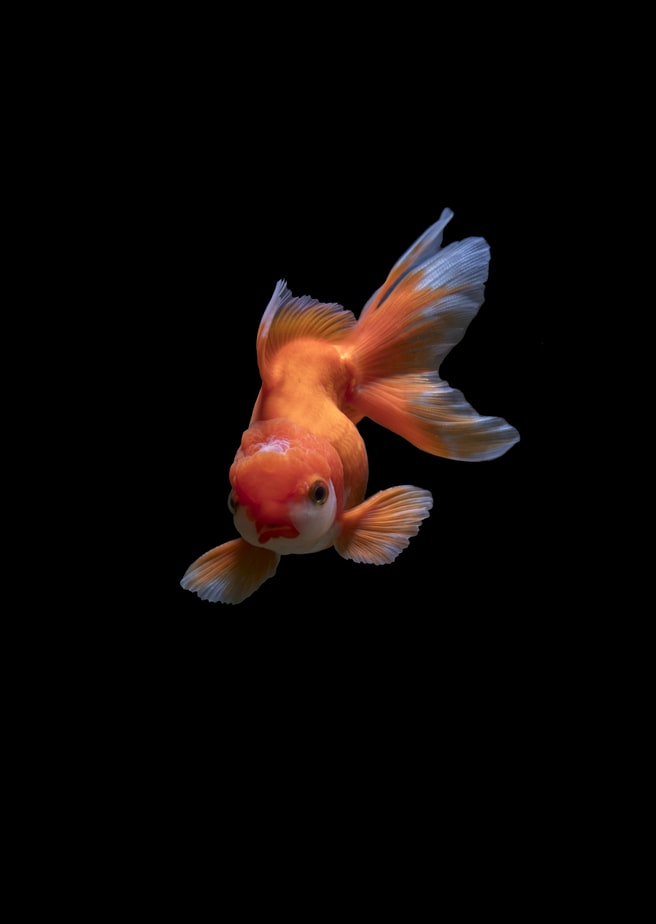
\includegraphics[width=6cm]{images/goldfish_zhengtaoTang}
	\end{columns}
	\begin{center}
		\Huge\color{tumwhite}
		\vfill\raggedleft
		{\small \color{tumgray} Photo by zhengtao tang on Unsplash}
		
	\end{center}
	\vfill
\end{frame}
}

\begin{frame}
	\frametitle{Attention}
	
	\begin{columns}
		\column{.5\textwidth}
		
%		
%		
%		\attention
%		
%		\attnv
		
		\begin{tikzpicture}[node distance=.2em]
		\node[label={below:$\V{\alpha}^T$}, draw=attentioncolor, rounded corners](alpha){\attention};
		\node[right=of alpha](out){\attnout};
		\node[above=of out, label={above:${\only<1,2>{\V{v}}\only<3>{\M{V}}}$}, draw=valuecolor, rounded corners]{\attnv};
		\visible<2->{
		\node[above=of alpha, label={above:$\M{K}$}, draw=keycolor, rounded corners]{\attnkey};
		\node[left=of alpha, label={below:${\only<1,2>{\V{q}}\only<3>{\M{Q}}}^T$}, draw=querycolor, rounded corners]{\attnquery};
		}
		\end{tikzpicture}
		
		%	\begin{equation*}
		%		\text{Attention}(Q,K,V) = 
		%		\begin{tikzpicture}
		%		\node(alpha){$\underbrace{\attention}_\alpha$};
		%		\node[right=of alpha](out){};
		%		\node[above=of out]{\attnv};
		%		\end{tikzpicture}
		%		 
		%	\end{equation*}
		
		
		\column{.5\textwidth}
		
		\begin{tikzpicture}[yscale=3]
			
			\visible<3>{
				\node[draw=valuecolor, circle, fill=valuecolor, fill opacity=.2, text opacity=1, font=\small, inner sep=.2em](d) at (1,.35){};
				\node[draw=valuecolor, circle, fill=valuecolor, fill opacity=.1, text opacity=1, font=\small, inner sep=.2em](e) at (2,.05){};
				\node[draw=valuecolor, circle, fill=valuecolor, fill opacity=.3, text opacity=1, font=\small, inner sep=.2em](f) at (3,.42){};
				\node[draw=valuecolor, circle, fill=valuecolor, fill opacity=.4, text opacity=1, font=\small, inner sep=.2em](g) at (4,.25){};
				\draw (d) -- (e) -- (f) -- (g);
			}
			
			\node[draw=valuecolor, circle, fill=valuecolor, fill opacity=.2, text opacity=1, font=\small, inner sep=.2em](a) at (1,.3){};
			\node[draw=valuecolor, circle, fill=valuecolor, fill opacity=.1, text opacity=1, font=\small, inner sep=.2em](b) at (2,.1){};
			\node[draw=valuecolor, circle, fill=valuecolor, fill opacity=.3, text opacity=1, font=\small, inner sep=.2em](c) at (3,.3){};
			\node[draw=valuecolor, circle, fill=valuecolor, fill opacity=.4, text opacity=1, font=\small, inner sep=.2em](d) at (4,.4){};
			
			\draw (a) -- (b) -- (c) -- (d);
			
			\foreach \t in {1,2,3,4} {
				\draw[tumgray] (\t,0) -- (\t,-.05) node[at end, below, text=tumgray] {$t_\t$};
			}
			
			%\draw[-stealth] (0,0) -- (0,.5);
			\draw[-stealth, tumgray] (.5,0) -- (4.5,0);
			
			\only<1,2>{
			\node[draw=tumblack, circle, fill=attentionoutcolor, text=white, fill opacity=1, text opacity=1, font=\small, inner sep=.2em, label={right:$\sum_{t=0}^{T} \alpha_t v_t = \V{\alpha}^T \V{v}$}](out) at (2.5,-.5) {};
			}
			\only<3>{
			\node[draw=white, circle, fill=attentionoutcolor, text=white, fill opacity=1, text opacity=1, font=\small, inner sep=.2em](outba) at (1.05,-.48) {};
			\node[draw=white, circle, fill=attentionoutcolor, text=white, fill opacity=1, text opacity=1, font=\small, inner sep=.2em](outbb) at (2.05,-.48) {};
			\node[draw=white, circle, fill=attentionoutcolor, text=white, fill opacity=1, text opacity=1, font=\small, inner sep=.2em](outbc) at (3.05,-.48) {};
			\node[draw=white, circle, fill=attentionoutcolor, text=white, fill opacity=1, text opacity=1, font=\small, inner sep=.2em](outbd) at (4.05,-.48) {};
				
			\node[draw=white, circle, fill=attentionoutcolor, text=white, fill opacity=1, text opacity=1, font=\small, inner sep=.2em](outa) at (1,-.5) {};
			\node[draw=white, circle, fill=attentionoutcolor, text=white, fill opacity=1, text opacity=1, font=\small, inner sep=.2em](out) at (2,-.5) {};
			\node[draw=white, circle, fill=attentionoutcolor, text=white, fill opacity=1, text opacity=1, font=\small, inner sep=.2em](outa) at (3,-.5) {};
			\node[draw=white, circle, fill=attentionoutcolor, text=white, fill opacity=1, text opacity=1, font=\small, inner sep=.2em](outa) at (4,-.5) {};

			}
		
			\node at (2.5, -.25) {};
			
			\draw[-stealth, draw=tumred, opacity=.4, line width=.4] (a) -- (out);
			\draw[-stealth, draw=tumred, opacity=.8, line width=.8] (b) -- (out);
			\draw[-stealth, draw=tumred, opacity=.2, line width=.2] (c) -- (out);
			\draw[-stealth, draw=tumred, opacity=.6, line width=.6] (d) -- (out);
			
			\node(annot1) at (5.5,.1){keep those};
			\draw[-stealth, tumred, shorten <= .3em, , shorten >= .3em](annot1) -- (b);
			\draw[-stealth, tumred, shorten <= .3em, , shorten >= .3em](annot1) -- (d);
			
			\node(annot2) at (3.5,.85){ignore these};
			\draw[-stealth, tumbluelight, shorten <= 1em, shorten >= 1em](annot2) -- (a);
			\draw[-stealth, tumbluelight, shorten <= 1em, shorten >= 1em](annot2) -- (c);
			
			
		\end{tikzpicture}
%		
%		
%		\begin{tikzpicture}
%		\begin{axis}[height=3cm,width=\textwidth,grid=major,]
%		\addplot coordinates {(0,.3) (1,.1) (2,.3) (3,.4)};
%		\end{axis}
%		\end{tikzpicture}
%		\begin{tikzpicture}
%			
%			\begin{axis}[ybar,height=3cm,width=\textwidth,grid=major,]
%			\addplot coordinates {(1,.05) (0,.4) (3,.05) (2,.5)};
%			\end{axis}
%		\end{tikzpicture}
	\end{columns}

	
	\Large
	\only<1>{
	\begin{equation*}
	\text{Attention}({\color{tumred}\V{\alpha}}, {\color{tumblue}\V{v}}) = {\color{tumred}\V{\alpha}}^T  {\color{tumblue}\V{v}} = \sum_{t=0}^{T} \alpha_tv_t, \quad \V{\alpha} \in [0,1]^{T=4}, \V{v} \in \mathbb{R}^{T}
	\end{equation*}
	}
	\only<2>{
		\begin{equation*}
		\text{Attention}({\color{tumorange}\V{K}}, {\color{tumgreen}\V{q}}, {\color{tumblue}\V{v}}) = 
		\overbrace{\text{softmax}\left({\color{tumgreen}\V{q}^T}{\color{tumorange}\V{K}}\right)}^{{\color{tumred}\V{\alpha}}^T}
		{\color{tumblue}\V{v}}, \quad \V{v} \in \mathbb{R}^{T}, \V{q} \in \mathbb{R}^{D_k}, \M{K} \in \mathbb{R}^{D_k \times T}
		\end{equation*}
	}
	\only<3>{
		\begin{equation*}
		\text{Attention}({\color{tumorange}\V{K}}, {\color{tumgreen}\V{Q}}, {\color{tumblue}\V{V}}) = 
		\text{softmax}\left({\color{tumgreen}\V{Q}^T}{\color{tumorange}\V{K}}\right)
		{\color{tumblue}\V{V}}, \quad \V{V} \in \mathbb{R}^{T \times D_v}, \V{Q} \in \mathbb{R}^{D_k \times T}, \M{K} \in \mathbb{R}^{D_k \times T}
		\end{equation*}
	}
\end{frame}


\begin{frame}
	
	
	\begin{equation*}
	\text{Attention}(Q,K,V) = \underbrace{\text{softmax}\left(QK^T\right)}_\alpha V
	\end{equation*}
	query: $Q \in \mathbb{R}^{t \times d_k}$
	
	key: $K \in \mathbb{R}^{t \times d_k}$
	
	value: $V \in \mathbb{R}^{t \times d_v}$
	
	attention scores $\alpha \in [0,1]^{t \times t}$
	
	
\end{frame}


\begin{frame}
	\frametitle{test}
	
	\tikzstyle{conn} = [-stealth, rounded corners, tumbluedark, thick]
	\tikzstyle{module} = [draw=none, fill=tumgraylight, rounded corners]
	\tikzstyle{layer} = [draw=none, fill=tumbluelight, rounded corners]
	
	\visible<2>{
	\begin{tikzpicture}[node distance=2em]
		\node(input){inputs};
		\node[below of=input](plus){+};
		\node[left of=plus](posenc){p};
		
		\node[module, below=2em of plus](attn){Multi-Head-Attention};
		\node[module, below=.5em of attn](addnorm){Add \& Norm};
		
		\node[module, below=2em of addnorm](ff){Feed Forward};
		\node[module, below=.5em of ff](addnorm2){Add \& Norm};
		
		
		\coordinate[above=of attn](in);
		\coordinate[below=of addnorm2](out);
		\draw[conn] (in) -- (attn);
		\draw[conn] (in) -- ($ (attn)!.5!(in) $) -| ($ (attn.north)+(2em,0) $);
		\draw[conn] (in) -- ($ (attn)!.5!(in) $) -| ($ (attn.north)-(2em,0) $);  
%		
		\draw[conn] (in) -- ($ (attn)!.6!(in) $) -| ($ (attn.east)+(.5em,0) $) |- (addnorm.east);

		\draw[conn] (attn) -- (addnorm);
		
		\draw[conn] (addnorm) -- (ff);
		\draw[conn] (addnorm) -- ($ (addnorm)!.5!(ff) $) -| ($ (ff.east)+(.5em,0) $) |- (addnorm2.east);
		\draw[conn] (ff) -- (addnorm2);
		\draw[conn] (addnorm2) -- (out);
		
		\begin{pgfonlayer}{background}
			\node[layer, draw=black, fit=(attn)(addnorm)(ff)(addnorm2)(in)(out)]{};
		\end{pgfonlayer}
		
	\end{tikzpicture}
}
	
\end{frame}


{\setbeamercolor{background canvas}{bg=tumblue}
	\begin{frame}[plain]
	\vfill
	\begin{center}
		\Huge\color{tumwhite}
		Results
	\end{center}
	\vfill
\end{frame}
}

\begin{frame}
	\frametitle{Preprocessed versus Raw Data (Sentinel 2, Region Holl)}
	
	\begin{tabular}{rrlrlrlrl}
		\toprule
		 & \multicolumn{2}{c}{MS-ResNet} & \multicolumn{2}{c}{RNN (LSTM)} & \multicolumn{2}{c}{Transformer} & \multicolumn{2}{c}{TempCNN} \\
		 & acc. & $\kappa$ & acc. & $\kappa$ & acc. & $\kappa$ & acc. & $\kappa$ \\
		\cmidrule(lr){2-3}\cmidrule(lr){4-5} \cmidrule(lr){6-7}\cmidrule(lr){8-9}
		preprocessed & \textbf{0.8654} & \textbf{0.8360} & 0.7997 & 0.7513 & \textbf{0.8647} & \textbf{0.8363} & \textbf{0.8407} & \textbf{0.8034} \\
		raw 		 & 0.8331 & 0.7971 & \textbf{0.8048} & \textbf{0.7611} & 0.7859 & 0.7420 & 0.7944 & 0.7462 \\
		\bottomrule
	\end{tabular}
	
%	\begin{tabular}{rllll}
%		\toprule
%		overall accuracy & MS-ResNet & RNN (LSTM) & Transformer & TempCNN \\
%		\cmidrule(lr){2-2}\cmidrule(lr){3-3}\cmidrule(lr){4-4}\cmidrule(lr){5-5}
%		preproc. (GAF) & 0.8654 & 0.7997 & 0.8647 & 0.8407 \\
%		raw & 0.8331 & 0.8048 & 0.7859 & 0.7944 \\
%		\bottomrule
%	\end{tabular}
	
	
	
	
\end{frame}

\begin{frame}
\frametitle{Preprocessed versus Raw Data (Sentinel 2, Region Holl)}

\begin{tabular}{lrlrlrlrl}
	\toprule
	& \multicolumn{2}{c}{MS-ResNet} & \multicolumn{2}{c}{RNN (LSTM)} & \multicolumn{2}{c}{Transformer} & \multicolumn{2}{c}{TempCNN} \\
	& acc. & $\kappa$ & acc. & $\kappa$ & acc. & $\kappa$ & acc. & $\kappa$ \\
	\cmidrule(lr){2-3}\cmidrule(lr){4-5} \cmidrule(lr){6-7}\cmidrule(lr){8-9}
	preprocessed & \textbf{0.8654} & \textbf{0.8360} & 0.7997 & 0.7513 & \textbf{0.8647} & \textbf{0.8363} & \textbf{0.8407} & \textbf{0.8034} \\
	raw 		 & 0.8331 & 0.7971 & \textbf{0.8048} & \textbf{0.7611} & 0.7859 & 0.7420 & 0.7944 & 0.7462 \\
	\bottomrule
\end{tabular}

\end{frame}

\begin{frame}
\frametitle{Radar}

\begin{tabular}{lrlrlrlrl}
	\toprule
	preprocessed data& \multicolumn{2}{c}{MS-ResNet} & \multicolumn{2}{c}{RNN (LSTM)} & \multicolumn{2}{c}{Transformer} & \multicolumn{2}{c}{TempCNN} \\
	& acc. & $\kappa$ & acc. & $\kappa$ & acc. & $\kappa$ & acc. & $\kappa$ \\
	\cmidrule(lr){2-3}\cmidrule(lr){4-5} \cmidrule(lr){6-7}\cmidrule(lr){8-9}
	Sentinel 1 + Sentinel 2 	& x & x & 0.7983 & 0.7503 & 0.8384 & 0.8037 & x & x \\
	Sentinel 2 (optical)	 	& x & x & 0.7845 & 0.7338 & 0.7936 & 0.7439 & x & x \\
	Sentinel 1 (radar)		 	& x & x & 0.7305 & 0.6608 & 0.7471 & 0.6861 & x & x \\
	\midrule \\
	raw data \\
	Sentinel 2 (optical) & 0.8331 & 0.7971 & \textbf{0.8048} & \textbf{0.7611} & 0.7859 & 0.7420 & 0.7944 & 0.7462 \\
\end{tabular}

\begin{tabular}{lrlrlrlrl}
	\toprule
	& \multicolumn{2}{c}{MS-ResNet} & \multicolumn{2}{c}{RNN (LSTM)} & \multicolumn{2}{c}{Transformer} & \multicolumn{2}{c}{TempCNN} \\
	& acc. & $\kappa$ & acc. & $\kappa$ & acc. & $\kappa$ & acc. & $\kappa$ \\
	\cmidrule(lr){2-3}\cmidrule(lr){4-5} \cmidrule(lr){6-7}\cmidrule(lr){8-9}
	raw (optical)		 & 0.8331 & 0.7971 & \textbf{0.8048} & \textbf{0.7611} & 0.7859 & 0.7420 & 0.7944 & 0.7462 \\
	\bottomrule
\end{tabular}

TODO experiments:
\begin{itemize}
	\item multiple runs and report standard deviation
	\item merge rows to one table
\end{itemize}

\end{frame}


%
\begin{frame}<presentation:4-5>
\frametitle{Let's look at a few Examples}
\framesubtitle{Sentinel 2 preprocessed by 
\includegraphics[width=4em]{images/GAF_logo}}


\begin{tikzpicture}[baseline=-2em, inner sep=0]

\begin{axis}[
width=\textwidth,
%	hide axis,
height=5.5cm,
ymin=0, ymax=1.2,
%no marks,  
draw opacity=.8,
smooth=0.001,
legend style={at={(.65,1.1)},line width=2pt, draw opacity=1},
legend columns=3,
ylabel={reflectance},
xlabel={time $t$}
]

\only<1,2>{
	\addplot[b2color, tsmark] table [x=t, y=B02, col sep=comma] {images/example/12-71456800.csv};
	\addplot[b3color, tsmark] table [x=t, y=B03, col sep=comma] {images/example/12-71456800.csv};
	\addplot[b4color, tsmark] table [x=t, y=B04, col sep=comma] {images/example/12-71456800.csv};
	\addplot[b5color, tsmark] table [x=t, y=B05, col sep=comma] {images/example/12-71456800.csv};
	\addplot[b6color, tsmark] table [x=t, y=B06, col sep=comma] {images/example/12-71456800.csv};
	\addplot[b7color, tsmark] table [x=t, y=B07, col sep=comma] {images/example/12-71456800.csv};
	\addplot[b8color, tsmark] table [x=t, y=B08, col sep=comma] {images/example/12-71456800.csv};
	\addplot[b8Acolor, tsmark] table [x=t, y=B8A, col sep=comma] {images/example/12-71456800.csv};
	\addplot[b11color, tsmark] table [x=t, y=B11, col sep=comma] {images/example/12-71456800.csv};
	\addplot[b12color, tsmark] table [x=t, y=B12, col sep=comma] {images/example/12-71456800.csv};
}
\only<2>{
	\node[font=\Large](classannot) at (axis cs:12,1.1) {\textbf{meadow} \small(parcel 71456800)};
}
\only<3>{
	\addplot[b2color, tsmark] table [x=t, y=B02, col sep=comma]  {images/example/12-71460758.csv};
	\addplot[b3color, tsmark] table [x=t, y=B03, col sep=comma]  {images/example/12-71460758.csv};
	\addplot[b4color, tsmark] table [x=t, y=B04, col sep=comma]  {images/example/12-71460758.csv};
	\addplot[b5color, tsmark] table [x=t, y=B05, col sep=comma]  {images/example/12-71460758.csv};
	\addplot[b6color, tsmark] table [x=t, y=B06, col sep=comma]  {images/example/12-71460758.csv};
	\addplot[b7color, tsmark] table [x=t, y=B07, col sep=comma]  {images/example/12-71460758.csv};
	\addplot[b8color, tsmark] table [x=t, y=B08, col sep=comma]  {images/example/12-71460758.csv};
	\addplot[b8Acolor, tsmark] table [x=t, y=B8A, col sep=comma] {images/example/12-71460758.csv};
	\addplot[b11color, tsmark] table [x=t, y=B11, col sep=comma] {images/example/12-71460758.csv};
	\addplot[b12color, tsmark] table [x=t, y=B12, col sep=comma] {images/example/12-71460758.csv};
	
	\node[font=\Large](classannot) at (axis cs:12,1.1) {\textbf{meadow} \small(parcel 71460758)};
}
\only<4>{
	\addplot[b2color, tsmark] table [x=t, y=B02, col sep=comma]  {images/example/12-71460855.csv};
	\addplot[b3color, tsmark] table [x=t, y=B03, col sep=comma]  {images/example/12-71460855.csv};
	\addplot[b4color, tsmark] table [x=t, y=B04, col sep=comma]  {images/example/12-71460855.csv};
	\addplot[b5color, tsmark] table [x=t, y=B05, col sep=comma]  {images/example/12-71460855.csv};
	\addplot[b6color, tsmark] table [x=t, y=B06, col sep=comma]  {images/example/12-71460855.csv};
	\addplot[b7color, tsmark] table [x=t, y=B07, col sep=comma]  {images/example/12-71460855.csv};
	\addplot[b8color, tsmark] table [x=t, y=B08, col sep=comma]  {images/example/12-71460855.csv};
	\addplot[b8Acolor, tsmark] table [x=t, y=B8A, col sep=comma] {images/example/12-71460855.csv};
	\addplot[b11color, tsmark] table [x=t, y=B11, col sep=comma] {images/example/12-71460855.csv};
	\addplot[b12color, tsmark] table [x=t, y=B12, col sep=comma] {images/example/12-71460855.csv};
	
	\node[font=\Large](classannot) at (axis cs:12,1.1) {\textbf{meadow} \small(parcel 71460855)};
}
\only<5>{
	\addplot[b2color, tsmark] table [x=t, y=B02, col sep=comma]  {images/example/27-71460091.csv};
	\addplot[b3color, tsmark] table [x=t, y=B03, col sep=comma]  {images/example/27-71460091.csv};
	\addplot[b4color, tsmark] table [x=t, y=B04, col sep=comma]  {images/example/27-71460091.csv};
	\addplot[b5color, tsmark] table [x=t, y=B05, col sep=comma]  {images/example/27-71460091.csv};
	\addplot[b6color, tsmark] table [x=t, y=B06, col sep=comma]  {images/example/27-71460091.csv};
	\addplot[b7color, tsmark] table [x=t, y=B07, col sep=comma]  {images/example/27-71460091.csv};
	\addplot[b8color, tsmark] table [x=t, y=B08, col sep=comma]  {images/example/27-71460091.csv};
	\addplot[b8Acolor, tsmark] table [x=t, y=B8A, col sep=comma] {images/example/27-71460091.csv};
	\addplot[b11color, tsmark] table [x=t, y=B11, col sep=comma] {images/example/27-71460091.csv};
	\addplot[b12color, tsmark] table [x=t, y=B12, col sep=comma] {images/example/27-71460091.csv};
	
	\node[font=\Large](classannot) at (axis cs:12,1.1) {\textbf{wheat} \small(parcel 71460091)};
}
\only<6>{
	\addplot[b2color, tsmark] table [x=t, y=B02, col sep=comma]  {images/example/27-71460294.csv};
	\addplot[b3color, tsmark] table [x=t, y=B03, col sep=comma]  {images/example/27-71460294.csv};
	\addplot[b4color, tsmark] table [x=t, y=B04, col sep=comma]  {images/example/27-71460294.csv};
	\addplot[b5color, tsmark] table [x=t, y=B05, col sep=comma]  {images/example/27-71460294.csv};
	\addplot[b6color, tsmark] table [x=t, y=B06, col sep=comma]  {images/example/27-71460294.csv};
	\addplot[b7color, tsmark] table [x=t, y=B07, col sep=comma]  {images/example/27-71460294.csv};
	\addplot[b8color, tsmark] table [x=t, y=B08, col sep=comma]  {images/example/27-71460294.csv};
	\addplot[b8Acolor, tsmark] table [x=t, y=B8A, col sep=comma] {images/example/27-71460294.csv};
	\addplot[b11color, tsmark] table [x=t, y=B11, col sep=comma] {images/example/27-71460294.csv};
	\addplot[b12color, tsmark] table [x=t, y=B12, col sep=comma] {images/example/27-71460294.csv};
	
	\node[font=\Large](classannot) at (axis cs:12,1.1) {\textbf{wheat} \small(parcel 71460294)};
}
\only<7-8>{
	\addplot[b2color, tsmark] table [x=t, y=B02, col sep=comma]  {images/example/12-71459194.csv};
	\addplot[b3color, tsmark] table [x=t, y=B03, col sep=comma]  {images/example/12-71459194.csv};
	\addplot[b4color, tsmark] table [x=t, y=B04, col sep=comma]  {images/example/12-71459194.csv};
	\addplot[b5color, tsmark] table [x=t, y=B05, col sep=comma]  {images/example/12-71459194.csv};
	\addplot[b6color, tsmark] table [x=t, y=B06, col sep=comma]  {images/example/12-71459194.csv};
	\addplot[b7color, tsmark] table [x=t, y=B07, col sep=comma]  {images/example/12-71459194.csv};
	\addplot[b8color, tsmark] table [x=t, y=B08, col sep=comma]  {images/example/12-71459194.csv};
	\addplot[b8Acolor, tsmark] table [x=t, y=B8A, col sep=comma] {images/example/12-71459194.csv};
	\addplot[b11color, tsmark] table [x=t, y=B11, col sep=comma] {images/example/12-71459194.csv};
	\addplot[b12color, tsmark] table [x=t, y=B12, col sep=comma] {images/example/12-71459194.csv};
	
}
\only<7>{
	\node[font=\Huge](classannot) at (axis cs:12,1.1) {\textbf{meadow or wheat?}};
}
\only<8>{
	\node[font=\Large](classannot) at (axis cs:12,1.1) {\textbf{meadow} \small(parcel 71459194)};
}


%
\only<1>{
	\legend{B02 (blue),B03 (green),B04 (red),B05,B06,B07,B08,B8A,B11,B12}
}

\end{axis}

\end{tikzpicture}

\end{frame}
%\begin{frame}
%\frametitle{Qualitative Examples}
%%	\framesubtitle{ConvGRU with r=256 recurrent cells}
%\centering
%\begin{tikzpicture}
%\matrix (m) [matrix of nodes, ampersand replacement=\&, row sep=0pt, column sep=2mm]{
%	$\V{x}_{RGB,t}$ \& labels $\V{y}$ \& pred. $\hat{\V{y}}$ \& $H(\V{y},\hat{\V{y}}$) \& activation \& activation \& activation \& activation
%	\tileexample{16494}{maize}{maize}{meadow}{meadow}{peas}{peas}{rape}{rape}
%	\tileexample{8133}{winter_spelt}{spelt}{winter_wheat}{wheat}{summer_barley}{s.barley}{maize}{maize}
%	\tileexample{12894}{meadow}{meadow}{winter_wheat}{wheat}{potatoe}{potato}{maize}{maize}
%	%		\tileexample{1823}{meadow}{meadow}{winter_wheat}{wheat}{summer_oat}{oat}{maize}{maize}
%	\\
%};
%\makeexamplelegend
%\end{tikzpicture}
%\end{frame}

%\begin{frame}
%\frametitle{Qualitative Examples}
%%	\framesubtitle{ConvGRU with r=256 recurrent cells}
%\centering
%\begin{tikzpicture}
%\matrix (m) [matrix of nodes, ampersand replacement=\&, row sep=0pt, column sep=2mm]{
%$\V{x}_{RGB,t}$ \& labels $\V{y}$ \& pred. $\hat{\V{y}}$ \& $H(\V{y},\hat{\V{y}}$) \& activation \& activation \& activation \& activation
%\tileexample{10879}{winter_rye}{rye}{winter_triticale}{triticale}{summer_barley}{s.barley}{winter_barley}{w.barley}
%\tileexample{10792}{winter_rye}{rye}{winter_wheat}{wheat}{winter_triticale}{triticale}{summer_barley}{s.barley}
%%		\tileexample{10969}{winter_wheat}{wheat}{winter_triticale}{triticale}{winter_rye}{rye}{rape}{rape}
%\tileexample{172}{winter_wheat}{wheat}{meadow}{meadow}{maize}{maize}{winter_barley}{w.barley}
%\\
%};
%\makeexamplelegend
%\end{tikzpicture}
%\end{frame}


%\begin{frame}
%\frametitle{How did the ConvRNN handle the cloud noise?}
%
%We performed two experiments
%\begin{enumerate}
%	\item Visualization of internal network states. We found some hidden states that were sensitive 
%\end{enumerate}
%
%\end{frame}




%\begin{frame}
%\frametitle{Looking back at the Unreasonable Effectiveness of RNNs Blog}
%\texttt{http://karpathy.github.io/2015/05/21/rnn-effectiveness/}
%\includegraphics[width=\textwidth]{images/karpathy_charrnn}
%\end{frame}

%\input{images/activations.tikz}
%\begin{frame}
%\frametitle{Cloud Sensitive Cells}
%\framesubtitle{LSTM cell \textbf{47} of 256}
%\figactivations{1}{47}
%\end{frame}
%
%\begin{frame}
%\frametitle{Ablation Experiment on Cloudy Data}
%\input{images/clouds.tikz}
%\end{frame}

\begin{frame}[c]
\frametitle{Publications and Code}
\centering 

\Large



Github + DockerHub

\vspace{1ex}


\includegraphics[width=2cm]{images/github} \hspace{.5ex}
\includegraphics[width=2cm]{images/qr_github} \hspace{.5ex}
\includegraphics[width=2cm]{images/docker}

\vspace{1ex}

\url{https://github.com/TUM-LMF/MTLCC}

\url{https://github.com/TUM-LMF/MTLCC-pytorch}

\vspace{1em}
\small
\textsl{
	Rußwurm M., Körner M. (2018). \textbf{Multi-Temporal Land Cover Classification with Sequential Recurrent Encoders}. ISPRS International Journal of Geo-Information. https://arxiv.org/abs/1802.02080.
}
	
\end{frame}

\end{document}


